% Options for packages loaded elsewhere
\PassOptionsToPackage{unicode}{hyperref}
\PassOptionsToPackage{hyphens}{url}
%
\documentclass[
]{article}
\usepackage{amsmath,amssymb}
\usepackage{lmodern}
\usepackage{ifxetex,ifluatex}
\ifnum 0\ifxetex 1\fi\ifluatex 1\fi=0 % if pdftex
  \usepackage[T1]{fontenc}
  \usepackage[utf8]{inputenc}
  \usepackage{textcomp} % provide euro and other symbols
\else % if luatex or xetex
  \usepackage{unicode-math}
  \defaultfontfeatures{Scale=MatchLowercase}
  \defaultfontfeatures[\rmfamily]{Ligatures=TeX,Scale=1}
\fi
% Use upquote if available, for straight quotes in verbatim environments
\IfFileExists{upquote.sty}{\usepackage{upquote}}{}
\IfFileExists{microtype.sty}{% use microtype if available
  \usepackage[]{microtype}
  \UseMicrotypeSet[protrusion]{basicmath} % disable protrusion for tt fonts
}{}
\makeatletter
\@ifundefined{KOMAClassName}{% if non-KOMA class
  \IfFileExists{parskip.sty}{%
    \usepackage{parskip}
  }{% else
    \setlength{\parindent}{0pt}
    \setlength{\parskip}{6pt plus 2pt minus 1pt}}
}{% if KOMA class
  \KOMAoptions{parskip=half}}
\makeatother
\usepackage{xcolor}
\IfFileExists{xurl.sty}{\usepackage{xurl}}{} % add URL line breaks if available
\IfFileExists{bookmark.sty}{\usepackage{bookmark}}{\usepackage{hyperref}}
\hypersetup{
  pdftitle={Substitution of red meat with legumes and risk of primary liver cancer in UK Biobank participants: a prospective cohort study},
  pdfauthor={Supplementary materials},
  hidelinks,
  pdfcreator={LaTeX via pandoc}}
\urlstyle{same} % disable monospaced font for URLs
\usepackage[margin=1in]{geometry}
\usepackage{longtable,booktabs,array}
\usepackage{calc} % for calculating minipage widths
% Correct order of tables after \paragraph or \subparagraph
\usepackage{etoolbox}
\makeatletter
\patchcmd\longtable{\par}{\if@noskipsec\mbox{}\fi\par}{}{}
\makeatother
% Allow footnotes in longtable head/foot
\IfFileExists{footnotehyper.sty}{\usepackage{footnotehyper}}{\usepackage{footnote}}
\makesavenoteenv{longtable}
\usepackage{graphicx}
\makeatletter
\def\maxwidth{\ifdim\Gin@nat@width>\linewidth\linewidth\else\Gin@nat@width\fi}
\def\maxheight{\ifdim\Gin@nat@height>\textheight\textheight\else\Gin@nat@height\fi}
\makeatother
% Scale images if necessary, so that they will not overflow the page
% margins by default, and it is still possible to overwrite the defaults
% using explicit options in \includegraphics[width, height, ...]{}
\setkeys{Gin}{width=\maxwidth,height=\maxheight,keepaspectratio}
% Set default figure placement to htbp
\makeatletter
\def\fps@figure{htbp}
\makeatother
\setlength{\emergencystretch}{3em} % prevent overfull lines
\providecommand{\tightlist}{%
  \setlength{\itemsep}{0pt}\setlength{\parskip}{0pt}}
\setcounter{secnumdepth}{5}
\usepackage{rotating}
\usepackage{caption}
\captionsetup{font=small,justification=raggedright,singlelinecheck=false}
\captionsetup[table]{labelformat=default, labelsep=period}
\captionsetup[figure]{labelformat=default, labelsep=period}
\renewcommand{\thetable}{S\arabic{table}}
\renewcommand{\thefigure}{S\arabic{figure}}
\usepackage{booktabs}
\usepackage{caption}
\usepackage{longtable}
\usepackage{rotating}
\usepackage{colortbl}
\usepackage{array}
\usepackage{anyfontsize}
\ifluatex
  \usepackage{selnolig}  % disable illegal ligatures
\fi

\title{Substitution of red meat with legumes and risk of primary liver cancer in UK Biobank participants: a prospective cohort study}
\author{Supplementary materials}
\date{}

\begin{document}
\maketitle

\begin{table}[t]
\caption{\label{tab:food-group}\textbf{Supplementary table 1. Summary of included foods for each food group.}} 
\fontsize{9.0pt}{10.8pt}\selectfont
\begin{tabular*}{1\linewidth}{@{\extracolsep{\fill}}>{\raggedright\arraybackslash}p{\dimexpr 0.2\linewidth-2\tabcolsep-1.5\arrayrulewidth}>{\raggedright\arraybackslash}p{\dimexpr 0.8\linewidth-2\tabcolsep-1.5\arrayrulewidth}}
\toprule
\textbf{Food group} & \textbf{Includes} \\ 
\midrule\addlinespace[2.5pt]
{\bfseries Legumes} & Soy-based desserts, baked beans, pulses, soy drinks (including calcium fortified),
  tofu-based products, hummus, peas \\ 
{\bfseries Red meat} & Beef, lamb, other meat including offal, pork \\ 
{\bfseries Processed meat} & Sausages, bacon (with and without fat), ham, liver pate \\ 
{\bfseries Animal-based foods} & Poultry, fish, dairy, eggs, mixed dishes, and sauces and condiments \\ 
{\bfseries Healthy plant-based foods} & Whole grains, fruits, nuts, plant oils, beverages (water, tea and coffee), vegetables \\ 
{\bfseries Unhealthy plant-based foods} & Refined cereals, potatoes, fruit juice, mixed dishes (vegetarian), sweets \& snacks, and sugar sweetened beverages \\ 
{\bfseries Alcoholic beverages} & Beer and cider, spirits and other alcoholic drinks, fortified wine, red and rose wine, white wine \\ 
\bottomrule
\end{tabular*}
\end{table}

\clearpage

\begin{table}[t]
\caption{\label{tab:cancer}\textbf{Replacing 15 g/day of total meat, red meat and processed meat with legumes and hazard ratios and 95\% confidence intervals for hepatocellular carcinoma and intrahepatic cholangiocarcinoma.}} 
\fontsize{9.0pt}{10.8pt}\selectfont
\begin{tabular*}{1\linewidth}{@{\extracolsep{\fill}}lcc}
\toprule
 & \textbf{Model 1}\textsuperscript{\textit{1}} & \textbf{Model 2}\textsuperscript{\textit{2}} \\ 
\cmidrule(lr){2-2} \cmidrule(lr){3-3}
\textbf{15 g/day of legumes replacing:} & \textbf{HR} \textbf{(95\% CI)} & \textbf{HR} \textbf{(95\% CI)} \\ 
\midrule\addlinespace[2.5pt]
\multicolumn{3}{l}{{\bfseries Hepatocellular carcinoma (n = 87)}} \\ 
\midrule\addlinespace[2.5pt]
Total red meat & 1.02 (0.94-1.11) & 1.06 (0.97-1.16) \\ 
Unprocessed red meat & 1.02 (0.93-1.11) & 1.04 (0.95-1.15) \\ 
Processed red meat & 1.04 (0.90-1.19) & 1.10 (0.96-1.27) \\ 
\midrule\addlinespace[2.5pt]
\multicolumn{3}{l}{{\bfseries Intrahepatic cholangiocarcinoma (n = 100)}} \\ 
\midrule\addlinespace[2.5pt]
Total red meat & 0.94 (0.87-1.02) & 0.97 (0.89-1.05) \\ 
Unprocessed red meat & 0.92 (0.85-1.00) & 0.94 (0.87-1.02) \\ 
Processed red meat & 1.03 (0.90-1.18) & 1.07 (0.93-1.23) \\ 
\bottomrule
\end{tabular*}
\begin{minipage}{\linewidth}
\textsuperscript{\textit{1}}Multivariate Cox proportional hazards regression model adjusted for age (as underlying timescale), other food groups, and total food intake, and additionally stratified on sex, age, and attended assessment centre.\\
\textsuperscript{\textit{2}}Further adjusted for educational level, Townsend deprivation index, living alone, physical activity, smoking, alcohol intake, and waist circumference.\\
\end{minipage}
\end{table}

\clearpage

\begin{table}[t]
\caption{\label{tab:legume}\textbf{No intake of legumes vs. quartiles of daily legume intake and hazard ratios and 95\% confidence intervals for primary liver cancer.}} 
\fontsize{9.0pt}{10.8pt}\selectfont
\begin{tabular*}{1\linewidth}{@{\extracolsep{\fill}}lccc}
\toprule
 &  & \textbf{Model 1}\textsuperscript{\textit{1}} & \textbf{Model 2}\textsuperscript{\textit{2}} \\ 
\cmidrule(lr){3-3} \cmidrule(lr){4-4}
\textbf{Characteristic} & \textbf{Mean daily legume intake} & \textbf{HR} \textbf{(95\% CI)} & \textbf{HR} \textbf{(95\% CI)} \\ 
\midrule\addlinespace[2.5pt]
Categories: &  &  &  \\ 
    No intake & 0.00 & — & — \\ 
    Q1 & 6.3 & 0.59 (0.35-0.98) & 0.60 (0.36-0.99) \\ 
    Q2 & 16 & 0.88 (0.57-1.35) & 0.90 (0.58-1.38) \\ 
    Q3 & 34 & 0.73 (0.46-1.17) & 0.74 (0.47-1.19) \\ 
    Q4 & 109 & 0.98 (0.64-1.52) & 1.07 (0.69-1.66) \\ 
\bottomrule
\end{tabular*}
\begin{minipage}{\linewidth}
\textsuperscript{\textit{1}}Multivariate Cox proportional hazards regression model adjusted for age (as underlying timescale), other food groups, and total food intake, and additionally stratified on sex, age, and attended assessment centre.\\
\textsuperscript{\textit{2}}Further adjusted for educational level, Townsend deprivation index, living alone, physical activity, smoking, alcohol intake, and waist circumference.\\
\end{minipage}
\end{table}

\clearpage

\begin{sidewaystable}[t]
\caption{\label{tab:sens}\textbf{Sensitivity analyses}} 
\fontsize{9.0pt}{10.8pt}\selectfont
\begin{tabular*}{1\linewidth}{@{\extracolsep{\fill}}>{\raggedright\arraybackslash}p{\dimexpr 0.111111111111111\linewidth-2\tabcolsep-1.5\arrayrulewidth}>{\centering\arraybackslash}p{\dimexpr 0.111111111111111\linewidth-2\tabcolsep-1.5\arrayrulewidth}>{\centering\arraybackslash}p{\dimexpr 0.111111111111111\linewidth-2\tabcolsep-1.5\arrayrulewidth}>{\centering\arraybackslash}p{\dimexpr 0.111111111111111\linewidth-2\tabcolsep-1.5\arrayrulewidth}>{\centering\arraybackslash}p{\dimexpr 0.111111111111111\linewidth-2\tabcolsep-1.5\arrayrulewidth}>{\centering\arraybackslash}p{\dimexpr 0.111111111111111\linewidth-2\tabcolsep-1.5\arrayrulewidth}>{\centering\arraybackslash}p{\dimexpr 0.111111111111111\linewidth-2\tabcolsep-1.5\arrayrulewidth}>{\centering\arraybackslash}p{\dimexpr 0.111111111111111\linewidth-2\tabcolsep-1.5\arrayrulewidth}>{\centering\arraybackslash}p{\dimexpr 0.111111111111111\linewidth-2\tabcolsep-1.5\arrayrulewidth}}
\toprule
 & \multicolumn{5}{c}{\textbf{Exclusion of participants with:}} &  & \multicolumn{2}{c}{\textbf{Exclusion of:}} \\ 
\cmidrule(lr){2-6} \cmidrule(lr){8-9}
 & \textbf{High alcohol intake}\textsuperscript{\textit{1}} & \textbf{Implausible food intake}\textsuperscript{\textit{2}} & \textbf{Liver disease before baseline}\textsuperscript{\textit{3}} & \textbf{Any cancer before baseline}\textsuperscript{\textit{4}} & \textbf{Fewer than 3 Oxford WebQs}\textsuperscript{\textit{5}} & \textbf{Death register as source of liver cancer events}\textsuperscript{\textit{6}} & \textbf{Waist circumference from analysis}\textsuperscript{\textit{7}} & \textbf{Soy milk from food substitutions}\textsuperscript{\textit{8}} \\ 
\cmidrule(lr){2-2} \cmidrule(lr){3-3} \cmidrule(lr){4-4} \cmidrule(lr){5-5} \cmidrule(lr){6-6} \cmidrule(lr){7-7} \cmidrule(lr){8-8} \cmidrule(lr){9-9}
\textbf{15 g/day of legumes replacing:} & \textbf{HR} \textbf{(95\% CI)} & \textbf{HR} \textbf{(95\% CI)} & \textbf{HR} \textbf{(95\% CI)} & \textbf{HR} \textbf{(95\% CI)} & \textbf{HR} \textbf{(95\% CI)} & \textbf{HR} \textbf{(95\% CI)} & \textbf{HR} \textbf{(95\% CI)} & \textbf{HR} \textbf{(95\% CI)} \\ 
\midrule\addlinespace[2.5pt]
Total red meat & 1.00 (0.94-1.06) & 1.01 (0.95-1.07) & 0.99 (0.93-1.06) & 1.03 (0.96-1.11) & 1.04 (0.96-1.12) & 1.02 (0.96-1.08) & 1.00 (0.94-1.06) & 1.03 (0.94-1.12) \\ 
Unprocessed red meat & 0.98 (0.92-1.05) & 0.99 (0.93-1.05) & 0.97 (0.90-1.04) & 1.00 (0.93-1.08) & 1.02 (0.94-1.11) & 1.00 (0.94-1.07) & 0.98 (0.92-1.05) & 1.01 (0.92-1.11) \\ 
Processed red meat & 1.06 (0.95-1.18) & 1.08 (0.98-1.20) & 1.08 (0.96-1.20) & 1.15 (1.01-1.30) & 1.11 (0.97-1.27) & 1.07 (0.98-1.18) & 1.06 (0.96-1.17) & 1.11 (0.98-1.25) \\ 
\bottomrule
\end{tabular*}
\begin{minipage}{\linewidth}
\textsuperscript{\textit{1}}Exclusion of the upper decile of alcohol intake (g/day) by sex. n cases = 150.\\
\textsuperscript{\textit{2}}Exclusion of participants below the 2.5th percentile and above the 97.5th percentile of energy intake (kJ/day) by sex. n cases = 164.\\
\textsuperscript{\textit{3}}ICD10 codes: K70-79, B16-19, Z94.4, I85, I86.4, and E83.0-1. ICD9 codes: 5710-5745, 0700-0709, V427 and 2750-2751. n cases = 151.\\
\textsuperscript{\textit{4}}ICD10 codes: C00-C97 and D00-D48. ICD9 codes: 1400-2399. n cases = 129.\\
\textsuperscript{\textit{5}}n cases = 109.\\
\textsuperscript{\textit{6}}n cases = 183.\\
\textsuperscript{\textit{7}}n cases = 173.\\
\textsuperscript{\textit{8}}Soy milk was removed from the legumes food group and moved to the food group healthy plant-based foods. n cases = 173.\\
\end{minipage}
\end{sidewaystable}

\clearpage

\begin{figure*}[t]

{\centering 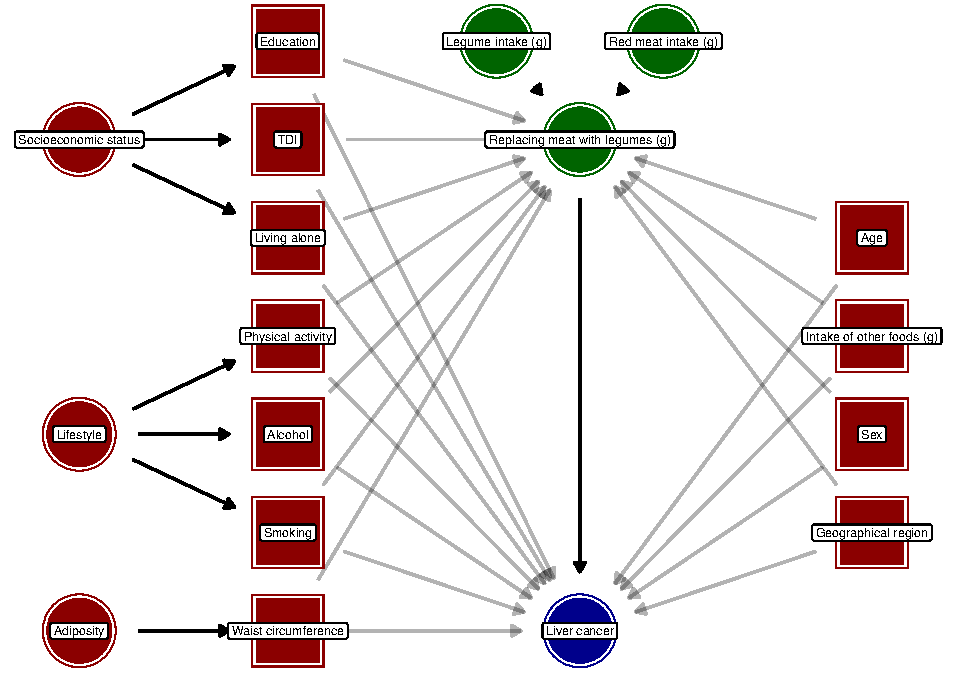
\includegraphics[width=1\linewidth,]{supplementary-materials_files/figure-latex/fig2-1} 

}

\caption{Simplified directed acyclic graph (DAG) visualizing the hypothesised causal relationship between replacing red meat with legumes and liver cancer based on assumptions of biasing paths. Red nodes represent confounders. Square nodes represent the minimal sufficient adjustment set for estimating the effect of replacing red meat with legumes on liver cancer. Shadowed arrows represent biasing paths. DAG terminology demands visualisation of all hypothesized correlating relationships between variables, typically resulting in complex and hard-to-follow illustrations. To improve readability, inter-covariate arrows are hidden in this DAG.}\label{fig:fig2}
\end{figure*}

\end{document}
